\documentclass[12pt, a4paper, oneside]{ctexart}
\usepackage{amsmath, amsthm, amssymb, bm, color, graphicx, geometry, mathrsfs,extarrows, braket, booktabs, array}
\usepackage[colorlinks,linkcolor=red,anchorcolor=blue,citecolor=blue,urlcolor=blue,menucolor=black]{hyperref}
\setmainfont{Times New Roman}  % 设置英文字体
\setsansfont{Calibri}
\setmonofont{Consolas}

\linespread{1.4}
%\geometry{left=2.54cm,right=2.54cm,top=3.18cm,bottom=3.18cm}
\geometry{left=1.84cm,right=1.84cm,top=2.18cm,bottom=2.18cm}
\newenvironment{problem}{\par\noindent\textbf{题目. }}{\bigskip\par}
\newenvironment{solution}{\par\noindent\textbf{解答. }}{\bigskip\par}
\newenvironment{note}{\par\noindent\textbf{注记. }}{\bigskip\par}

\everymath{\displaystyle} % 默认全部行间公式
\DeclareMathOperator*\uplim{\overline{lim}} % 定义上极限 \uplim_{}
\DeclareMathOperator*\lowlim{\underline{lim}} % 定义下极限 \lowlim_{}
\let\leq=\leqslant % 将全部leq变为leqslant
\let\geq=\geqslant % geq同理

% 一些宏定义
\def\bd{\boldsymbol}    % 加粗(向量) boldsymbol
\def\disp{\displaystyle}% 使用行间公式 displaystyle(默认)
\def\tsty{\textstyle}   % 使用行内公式 textstyle
\def\sign{\text{sign}}  % sign function
\def\wtd{\widetilde}    % 宽波浪线 widetilde
\def\R{\mathbb{R}}      % Real number
\def\C{\mathbb{C}}      % Complex number
\def\d{\mathrm{d}}      % differential operator
\def\e{\mathrm{e}}      % Euler's number
\def\i{\mathrm{i}}      % imaginary number
\def\re{\mathrm{Re\,}}    % Real part
\def\im{\mathrm{Im\,}}    % Imaginary part
\def\L{\mathcal{L}}     % Loss function
\def\wdh{\widehat}      % 宽帽子 widehat
\def\ol{\overline}      % 上横线 overline
\def\ul{\underline}     % 下横线 underline
\def\add{\vspace{1ex}}  % 增加行间距
\def\del{\vspace{-3.5ex}}  % 减少行间距

% 基本信息
\newcommand{\RQ}{\today} % 日期
\newcommand{\km}{最优化方法} % 科目
\newcommand{\bj}{强基数学002} % 班级
\newcommand{\xm}{吴天阳} % 姓名
\newcommand{\xh}{2204210460} % 学号

\begin{document}

%\pagestyle{empty}
\pagestyle{plain}
\vspace*{-15ex}
\centerline{\begin{tabular}{*5{c}}
    \parbox[t]{0.25\linewidth}{\begin{center}\textbf{日期}\\ \large \textcolor{blue}{\RQ}\end{center}} 
    & \parbox[t]{0.2\linewidth}{\begin{center}\textbf{科目}\\ \large \textcolor{blue}{\km}\end{center}}
    & \parbox[t]{0.2\linewidth}{\begin{center}\textbf{班级}\\ \large \textcolor{blue}{\bj}\end{center}}
    & \parbox[t]{0.1\linewidth}{\begin{center}\textbf{姓名}\\ \large \textcolor{blue}{\xm}\end{center}}
    & \parbox[t]{0.15\linewidth}{\begin{center}\textbf{学号}\\ \large \textcolor{blue}{\xh}\end{center}} \\ \hline
\end{tabular}}
\vspace*{4ex}

% 正文部分
\paragraph{第五章\ 习题3}设$f(x)=\frac{1}{2}\sum_{i=1}^4f_i(x)^2,\ r_i(x) = x_1e^{-x_2t_i}-y_i,\ i=1,2,3,4$, 其中$t_1=-1,t_2=0,t_3=1,t_4=2,y_1=2.7, y_2=1, y_3=0.4, y_4=0.1$.

(1) 以$x^{(1)} = (1,1)^T$为初始点, 计算进行一次Gauss-Newton迭代所得的点$x^{(2)}$;

(2) 在点$x^{(2)}$还是用矩阵$A_1^TA_1$进行一次近似的Gauss-Newton迭代得点$x^{(3)}$. 由这三个点估计方法对此问题的线性收敛速度.
\begin{solution}
    (1) \begin{equation*}
        A(x) = [\nabla r_1(x)\quad\nabla r_2(x)\quad\nabla r_3(x)\quad\nabla r_4(x)]^T = \left[\begin{matrix}
            e^{-x_2t_1}&-x_1t_1e^{-x_2t_1}\\
            e^{-x_2t_2}&-x_1t_2e^{-x_2t_2}\\
            e^{-x_2t_3}&-x_1t_3e^{-x_2t_3}\\
            e^{-x_2t_4}&-x_1t_4e^{-x_2t_4}\\
        \end{matrix}\right]
    \end{equation*}
    则$A_1 = A(x^{(1)}) = \left[\begin{matrix}
        e&1&e^{-1}&e^{-2}\\
        e&0&-e^{-1}&-2e^{-2}
    \end{matrix}\right]^T$, 于是
    \begin{equation*}
        \begin{aligned}
        A_1^TA_1 =&\ \left[\begin{matrix}
            e^2+1e^{-2}+e^{-4}&e^2-e^{-2}-2e^{-4}\\
            e^2-e^{-2}-2e^{-4}&e^2+e^{-2}+4e^{-4}
        \end{matrix}\right]\\
        A_1^Tr_1 =&\ \left[\begin{matrix}
        e&1&e^{-1}&e^{-2}\\
        e&0&-e^{-1}&-2e^{-2}
    \end{matrix}\right]^T\left[\begin{matrix}
        e-2.7\\0\\e^{-1}-0.4\\e^{-2}-0.1
    \end{matrix}\right]=\left[\begin{matrix}
        e^2-2.7e-0.4e^{-1}+0.9e^{-2}+e^{-4}\\
        e^2-2.7e+0.4e^{-1}-0.8e^{-2}-2e^{-4}
    \end{matrix}\right]
        \end{aligned}
    \end{equation*}
    求解$A_1^TA_1\delta_1 = A_1^Tr_1$, 得$\delta_1 = [-0.0040\quad 0.0106]^T$, 于是$x^{(2)} = x^{(1)}+\delta_1 = [0.9960\quad 1.0106]^T$.

    (2) 求解$A_1^TA_1\delta_2 = A_2^Tr_2$, 得$\delta_2 = [-0.0076\quad 0.0210]^T$,于是$x^{(3)} = x^{(2)} +\delta_2 = [0.9884\quad 1.0316]^T$.
\end{solution}
\paragraph{4.}写出下列等式的KKT条件.
\begin{equation*}
    \begin{aligned}
        &\ \min\quad q(x)=\frac{1}{2}x^TGx+x^Tg\\
        &\ s.t.\quad Ax\geq b,\qquad \ol{A}x=\ol{b}.
    \end{aligned}
\end{equation*}
其中$G$是对称正半定矩阵.
\begin{solution}
    设$A, \ol{A} \in \R^{m\times n}$, 则
    \begin{equation*}
        L(x,\lambda) = \frac{1}{2}x^TGx+x^Tg-\lambda_1^T(Ax-b)-\lambda_2^T(\ol{A}x-\ol{b}).
    \end{equation*}
    则KKT条件为
    \begin{equation*}
        \begin{cases}
            \frac{\partial L}{\partial x}(x^*) = Gx^*+g-A^T\lambda_1-\ol{A}^T\lambda_2 = 0,\\
            Ax^* \geq b,\\
            \ol{A}x^* = \ol{b},\\
            \lambda_1,\ \lambda_2\geq 0,\\
            \lambda_1^T(Ax^*-b) = 0.
        \end{cases}
    \end{equation*}
\end{solution}
\begin{problem}
    求下列规划问题的K-T点
    \begin{equation*}
        \left\{
            \begin{aligned}
                \min\quad f(x_1,x_2)=&\ (x_1-3)^2+(x_2-2)^2\\
                s.t.\quad g_1(x_1,x_2)=&\ x_1^2+x_2^2-5\leq 0\\
                g_2(x_1,x_2)=&\ x_1+2x_2-4\leq 0\\
                g_3(x_1,x_2)=&\ -x_1\leq 0\\
                g_4(x_1,x_2)=&\ -x_2\leq 0.
            \end{aligned}
        \right.
    \end{equation*}
\end{problem}
\begin{solution}
    \begin{equation*}
        L(f, \lambda) = (x_1-3)^2+(x_2-2)^2+\lambda_1(x_1^2+x_2^2-5)+\lambda_2(x_1+2x_2-4)+\lambda_3(-x_1)+\lambda_4(-x_2)
    \end{equation*}
    则KKT条件为
    \begin{equation*}
        \begin{cases}
            \frac{\partial L}{\partial x}(x^*) = \left[\begin{matrix}
                2(x_1-3)+2\lambda_1x_1+\lambda_2-\lambda_3\\
                2(x_2-3)+2\lambda_1x_2+2\lambda_2-\lambda_4
            \end{matrix}\right]=\left[\begin{matrix}
                0\\0
            \end{matrix}\right],\\
            x_1^2+x_2^2-5\leq 0,\\
            x_1+2x_2-4\leq 0,\\
            -x_1\leq 0,\\
            -x_2\leq 0,\\
            \lambda_1,\lambda_2,\lambda_3,\lambda_4\geq 0,\\
            \lambda_1(x_1^2+x_2^2-5)=0,\\
            \lambda_2(x_1+x_2-4) = 0,\\
            \lambda_3x_1=0,\\
            \lambda_4x_2=0.
        \end{cases}\Rightarrow
        \begin{cases}
            x_1 = 2,\quad x_2 = 1,\\
            \lambda_1 = \lambda_3 = \lambda_4 = 0,\\
            \lambda_2 = 0.
        \end{cases}
    \end{equation*}
    则K-T点为$x^* = [2\quad 1]^T$.
\end{solution}

% 下面给一些功能的写法
\iffalse
% 图片模板
\centerline{
    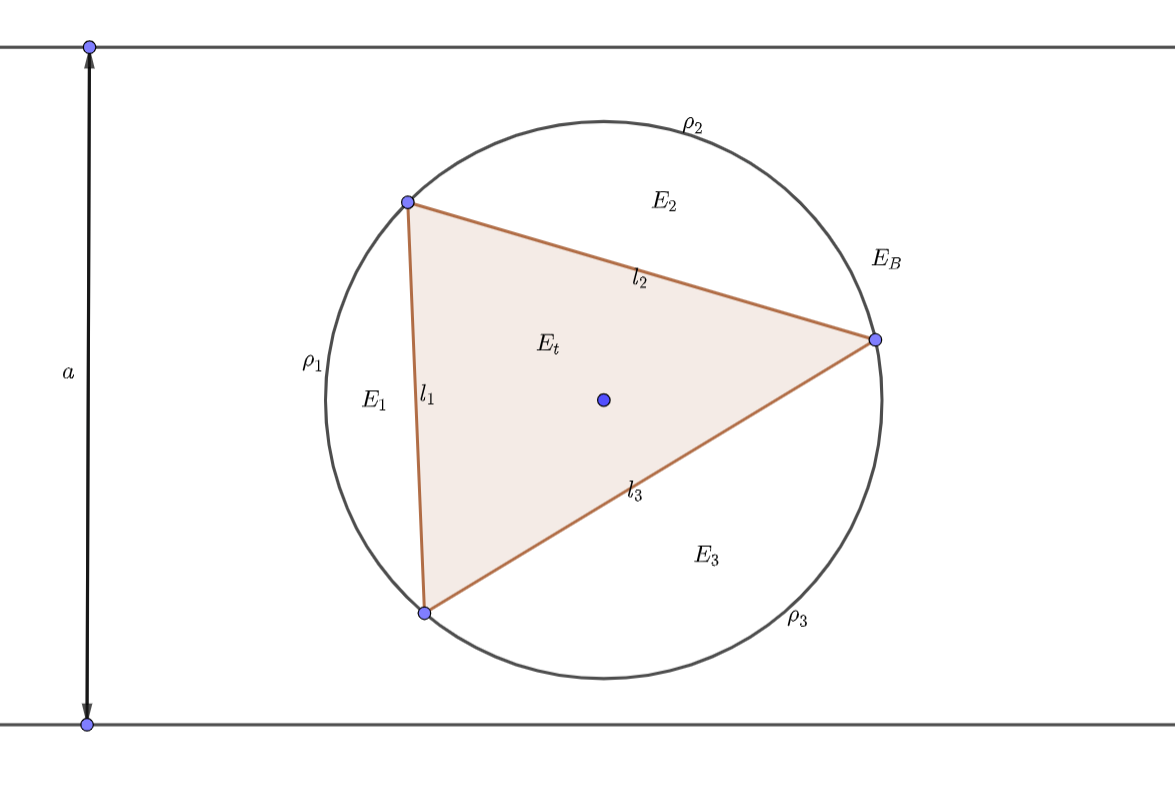
\includegraphics[width=0.8\textwidth]{figure.png}
}
% 表格模板
\renewcommand\arraystretch{0.8} % 设置表格高度为原来的0.8倍
\begin{table}[!htbp] % table标准
    \centering % 表格居中
    \begin{tabular}{p{1cm}<{\centering}p{1cm}<{\centering}p{3cm}<{\centering}p{5cm}<{\centering}} % 设置表格宽度
    %\begin{tabular}{cccc}
        \toprule
        $x_i$ & $f[x_1]$ & $f[x_i,x_{i+1}]$ & $f[x_i,x_{i+1},x_{i+2}]$ \\
        \midrule
        $x_0$ & $f(x_0)$ &                  &                          \\
        $x_0$ & $f(x_0)$ & $f'(x_0)$        &                          \\
        $x_0$ & $f(x_1)$ & $\frac{f(x_1)-f(x_0)}{x_1-x_0}$ & $\frac{f(x_1)-f(x_0)}{(x_1-x_0)^2}-\frac{f'(x_0)}{x_1-x_0}$\\
        \bottomrule
    \end{tabular}
\end{table}

\def\Log{\text{Log}} % 一个简单的宏定义
$\Log$ % 调用方法
\fi

\end{document}